\chapter{PANDUAN OPERASIONAL PENGGUNA (USER GUIDE)}

Bab ini menyajikan panduan langkah-demi-langkah penggunaan platform \textit{e-Learning} PT. BPR Jatim bagi kedua jenis pengguna: Administrator PSDM (melalui Portal Web) dan Karyawan (melalui Aplikasi Mobile). Setiap langkah dilengkapi dengan tangkapan layar (\textit{screenshot}) untuk mempermudah pemahaman.

\section{Panduan Web Administrator (Divisi PSDM)}
Portal Web Admin diakses oleh staf PSDM melalui peramban (\textit{browser}) menggunakan kredensial khusus administrator.

\subsection{Login Portal Web Admin}
\begin{enumerate}
    \item Buka peramban (\textit{browser}) dan akses alamat URL portal \textit{e-Learning} kantor.
    \item Masukkan email administrator dan kata sandi pada halaman login sebagaimana ditunjukkan pada Gambar \ref{fig:login_web}.
    \item Klik tombol \textbf{Masuk}. Jika kredensial valid, sistem akan mengarahkan pengguna ke halaman \textit{Dashboard} utama.
\end{enumerate}

\begin{figure}[H]
    \centering
    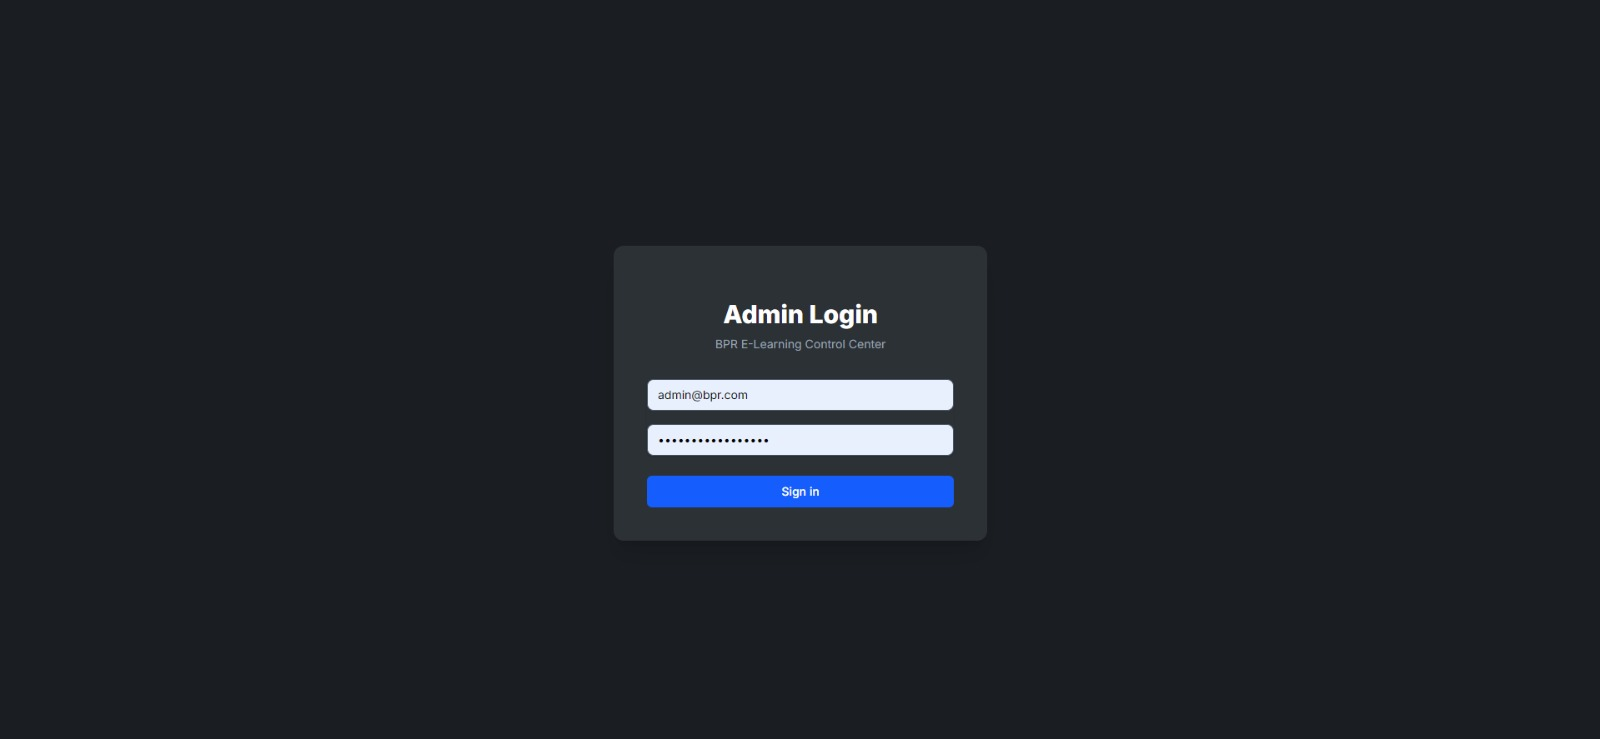
\includegraphics[width=0.85\textwidth]{image/loginweb.jpeg}
    \caption{Halaman Login Portal Web Administrator}
    \label{fig:login_web}
\end{figure}

\subsection{Dashboard Utama}
Setelah berhasil login, Admin akan melihat halaman \textit{Dashboard} utama yang menampilkan ringkasan statistik sistem, termasuk jumlah karyawan terdaftar, jumlah modul aktif, dan grafik analitik nilai kuis. Tampilan \textit{Dashboard} ditunjukkan pada Gambar \ref{fig:dashboard_web}.

\begin{figure}[H]
    \centering
    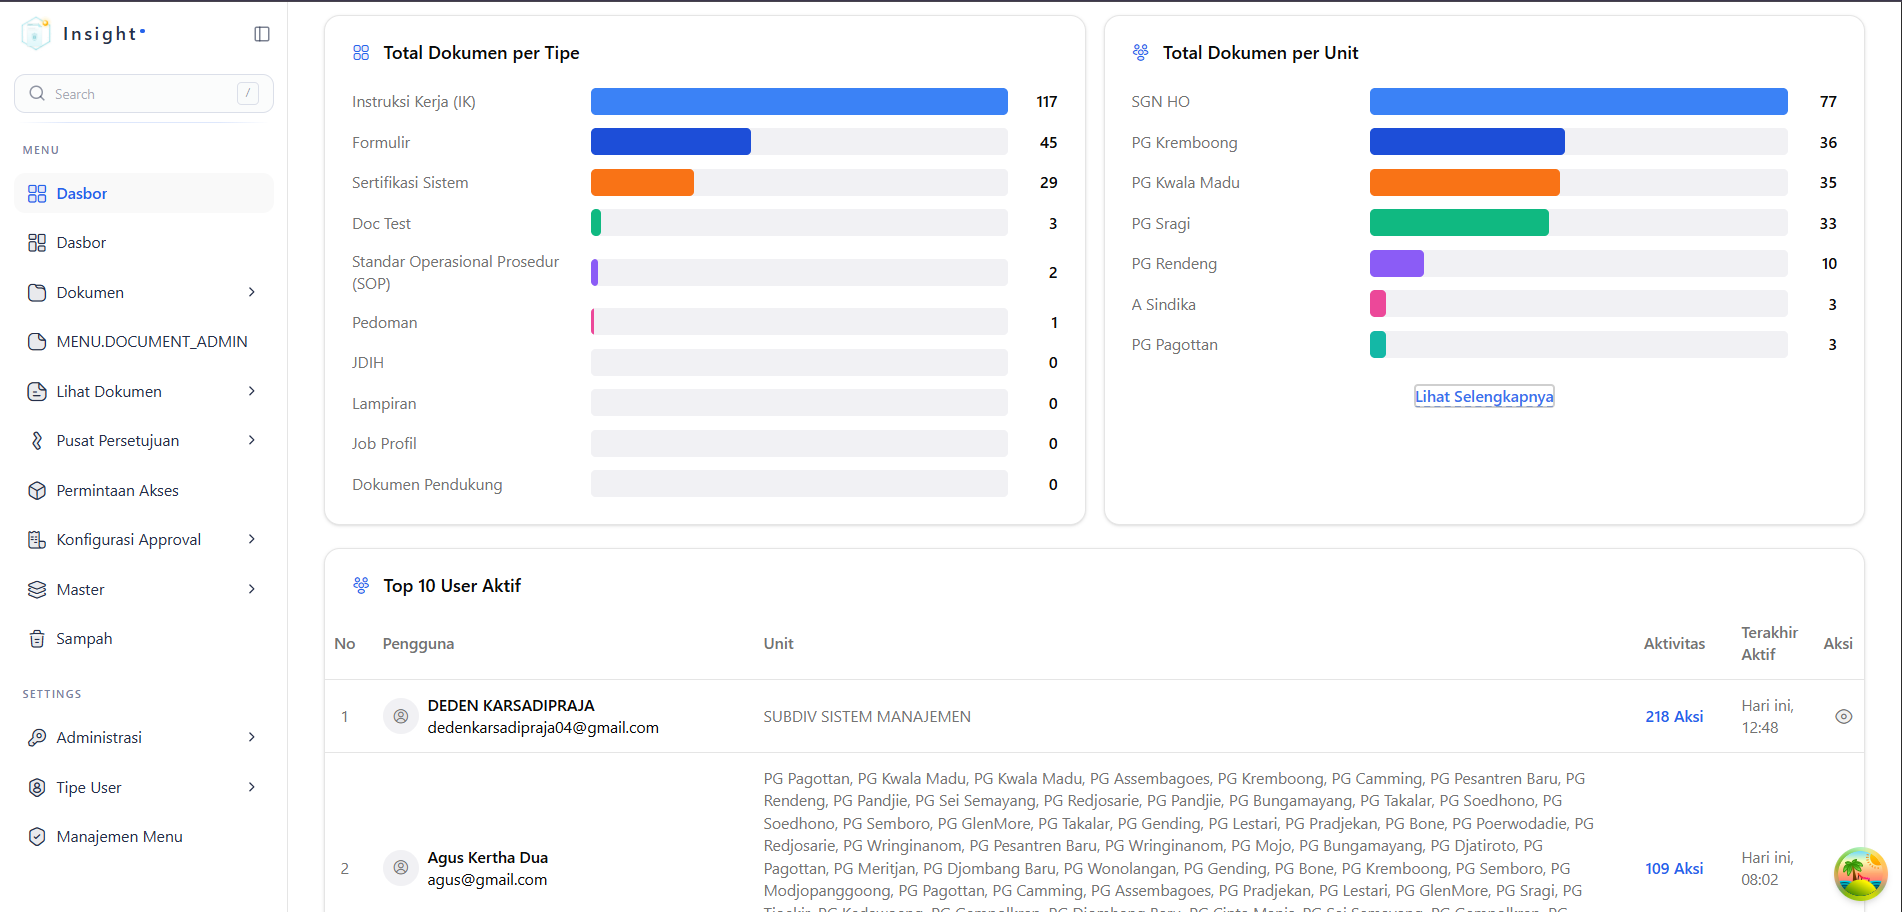
\includegraphics[width=0.85\textwidth]{image/dashboard-putih-pagination.png}
    \caption{Halaman Dashboard Utama Portal Web Admin}
    \label{fig:dashboard_web}
\end{figure}

\subsection{Manajemen Data Karyawan}
\begin{enumerate}
    \item Klik menu \textbf{Karyawan} pada \textit{sidebar} kiri untuk melihat daftar seluruh karyawan PT. BPR Jatim yang terdaftar (Gambar \ref{fig:kelola_karyawan}).
    \item Untuk menambah karyawan baru, klik tombol \textbf{Tambah Karyawan}, masukkan NIP, nama lengkap, divisi, email, dan \textit{password} bawaan (Gambar \ref{fig:tambah_karyawan}). Klik \textbf{Simpan}.
    \item Untuk mengedit data karyawan, klik ikon \textbf{Edit} pada baris karyawan yang ingin diubah. Lakukan perubahan data dan klik \textbf{Simpan}.
    \item Untuk menghapus karyawan, klik ikon \textbf{Hapus} dan konfirmasi penghapusan.
\end{enumerate}

\begin{figure}[H]
    \centering
    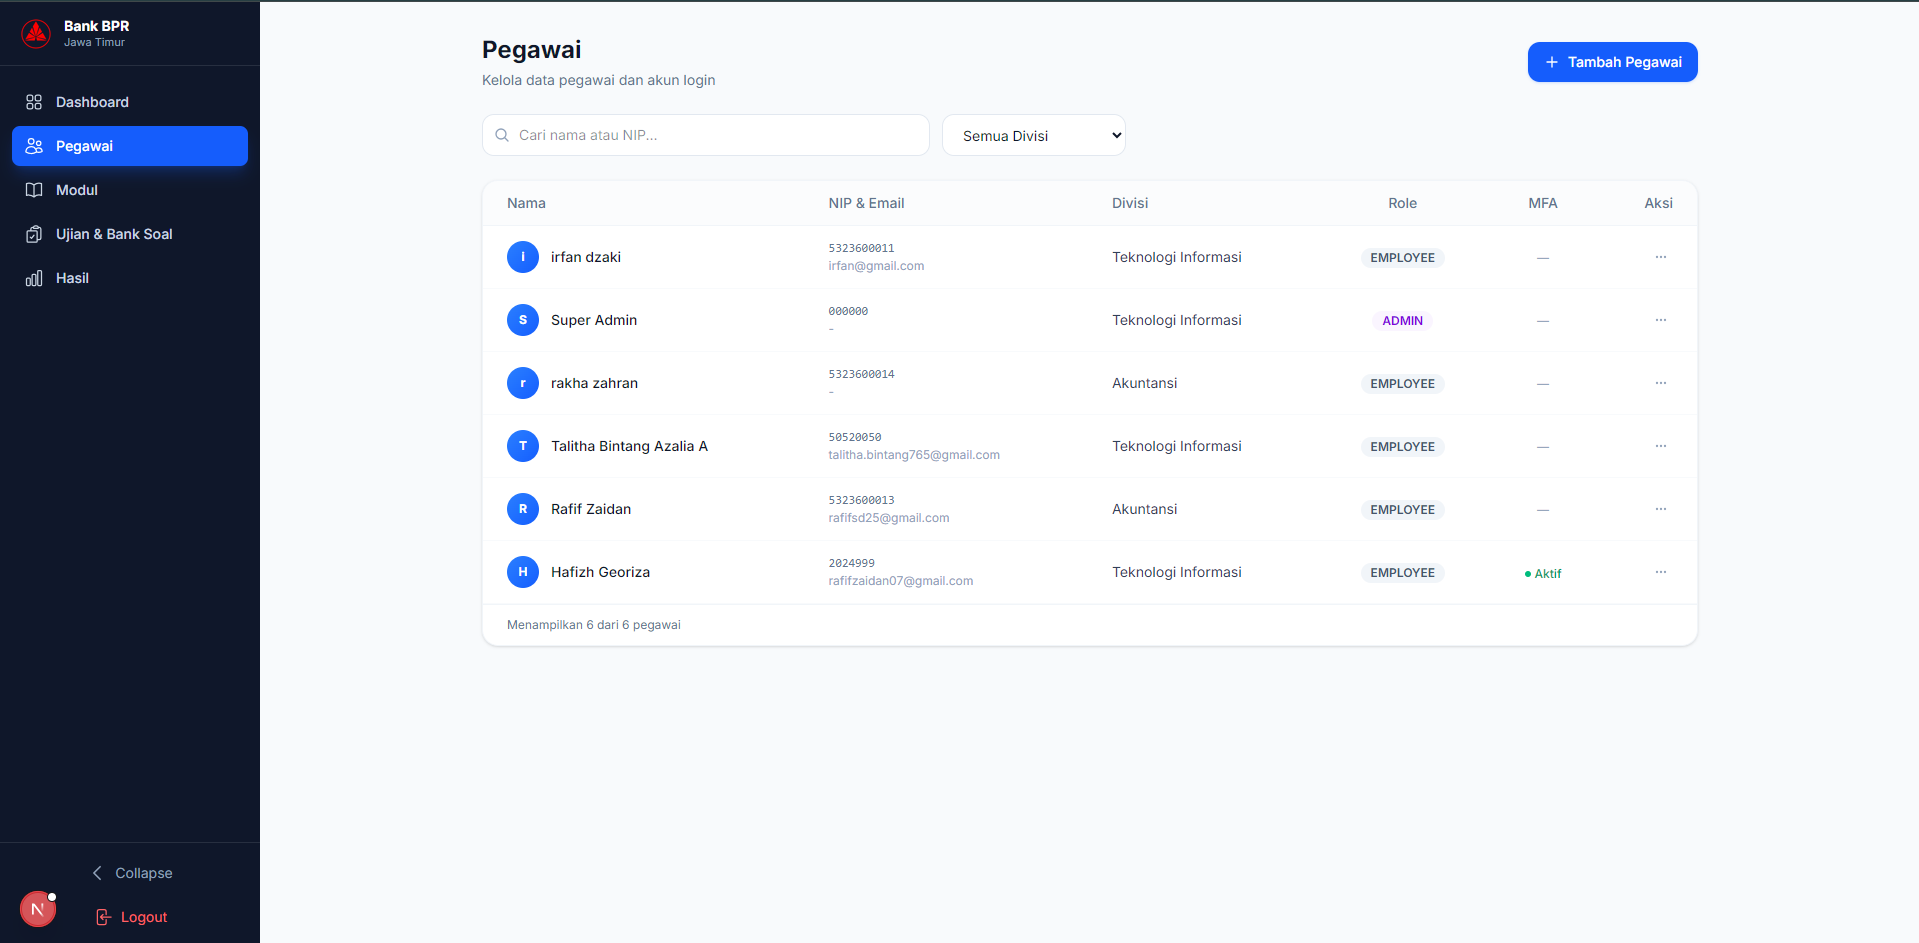
\includegraphics[width=0.85\textwidth]{image/halaman-kelola-karyawan.png}
    \caption{Halaman Kelola Data Karyawan}
    \label{fig:kelola_karyawan}
\end{figure}

\begin{figure}[H]
    \centering
    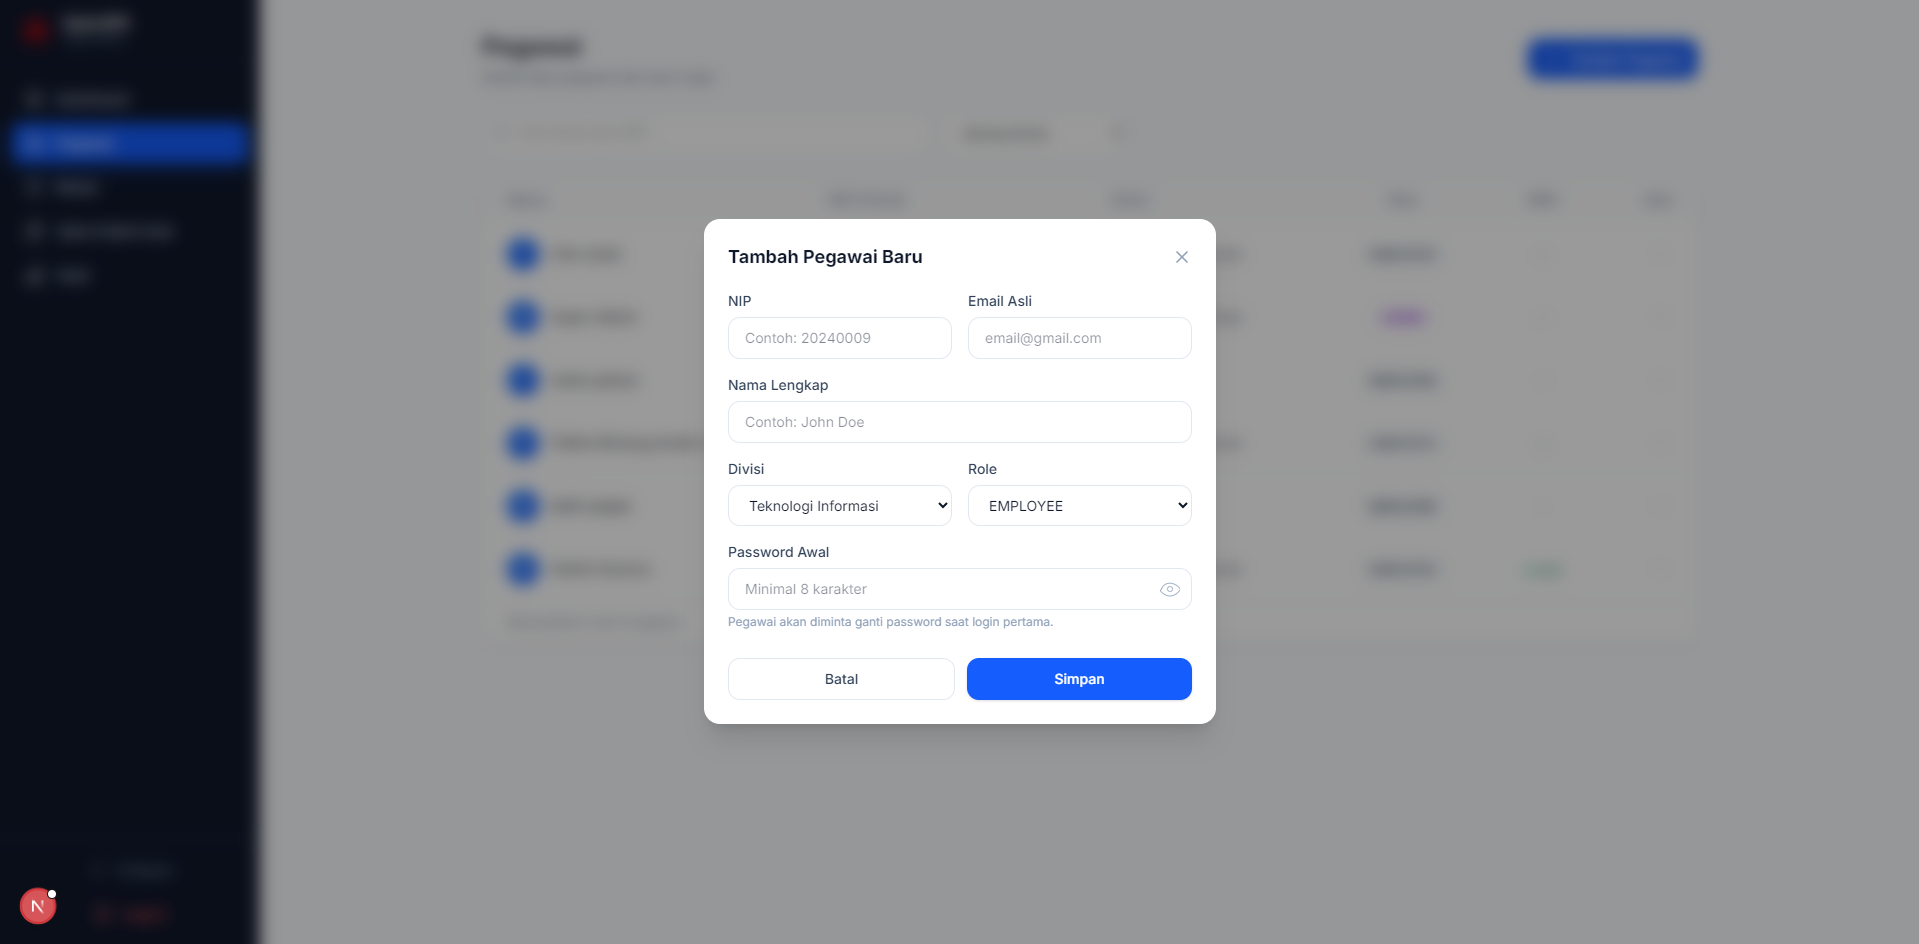
\includegraphics[width=0.75\textwidth]{image/fitur-tambah-pegawai.png}
    \caption{Form Tambah Data Karyawan Baru}
    \label{fig:tambah_karyawan}
\end{figure}

\subsection{Pengunggahan Modul Pembelajaran}
\begin{enumerate}
    \item Masuk ke menu \textbf{Kelola Materi} pada \textit{sidebar} kiri (Gambar \ref{fig:kelola_materi}).
    \item Klik \textbf{Unggah Modul Baru}.
    \item Masukkan judul modul, pilih divisi sasaran pelatihan, dan unggah berkas berformat PDF (Gambar \ref{fig:tambah_modul}).
    \item Klik \textbf{Simpan}. Berkas secara otomatis terunggah ke \textit{bucket} penyimpanan Supabase Storage dan dapat diakses langsung oleh karyawan sasaran.
\end{enumerate}

\begin{figure}[H]
    \centering
    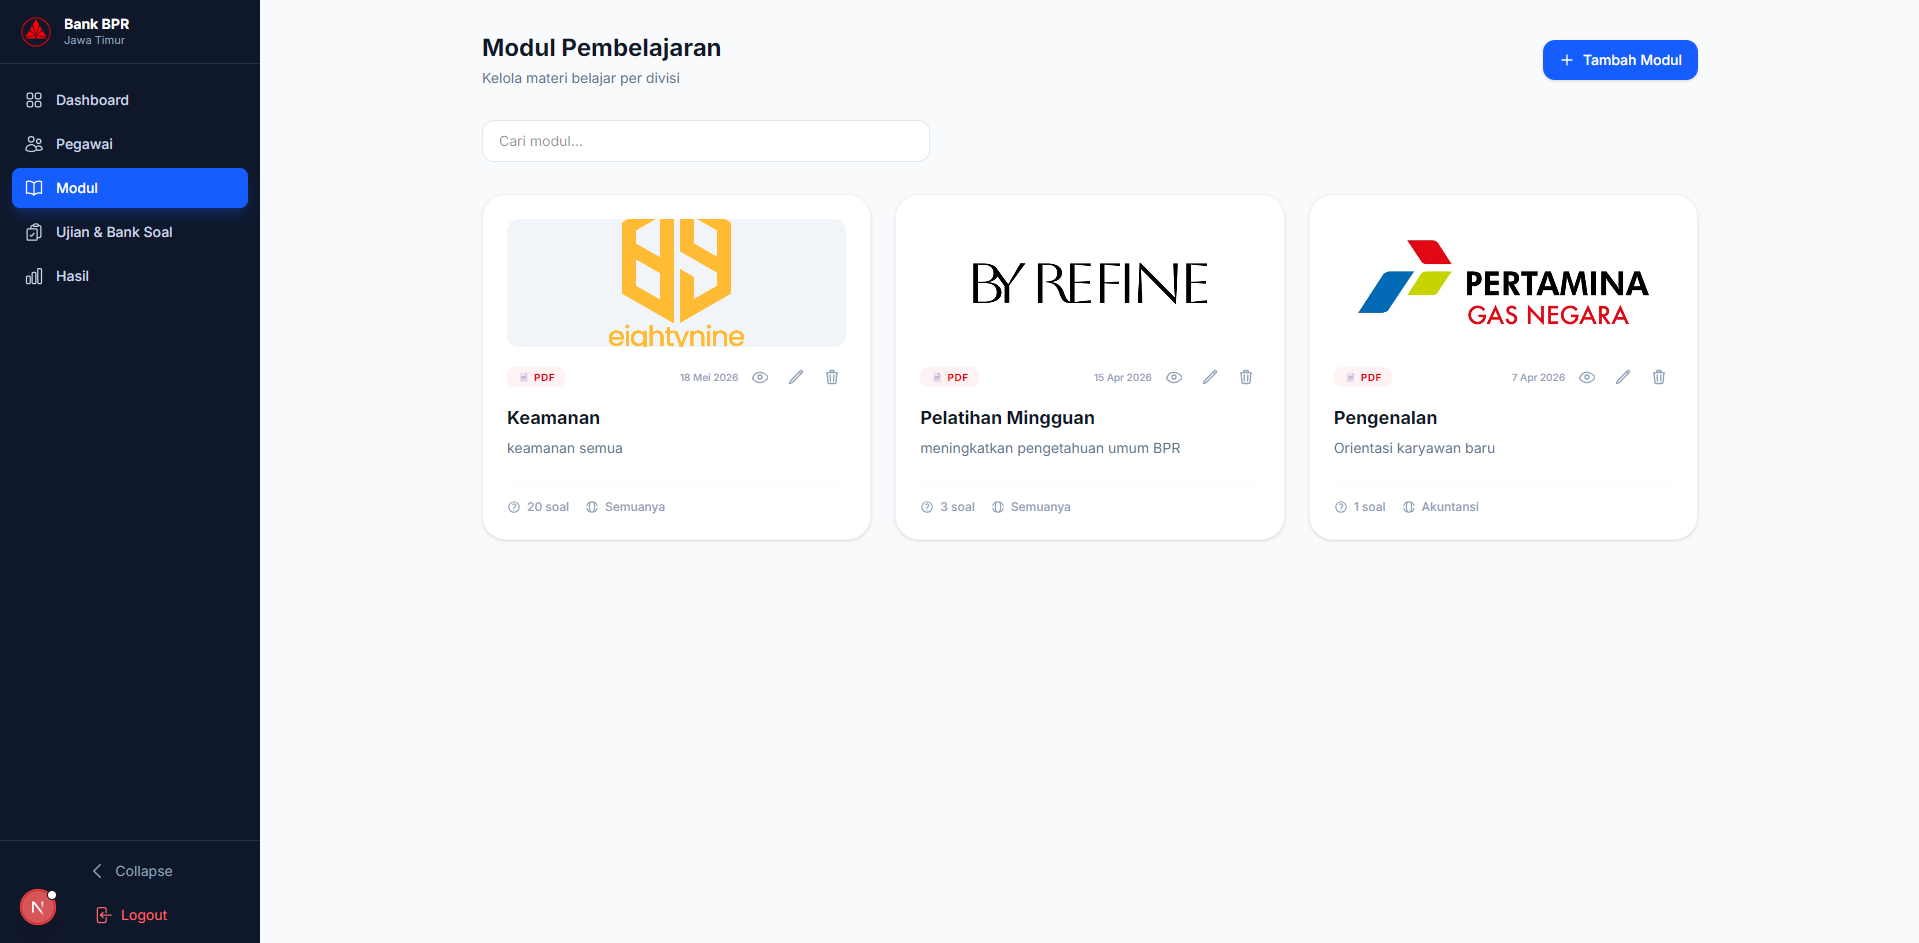
\includegraphics[width=0.85\textwidth]{image/halaman-kelola-materi.png}
    \caption{Halaman Kelola Materi Pelatihan}
    \label{fig:kelola_materi}
\end{figure}

\begin{figure}[H]
    \centering
    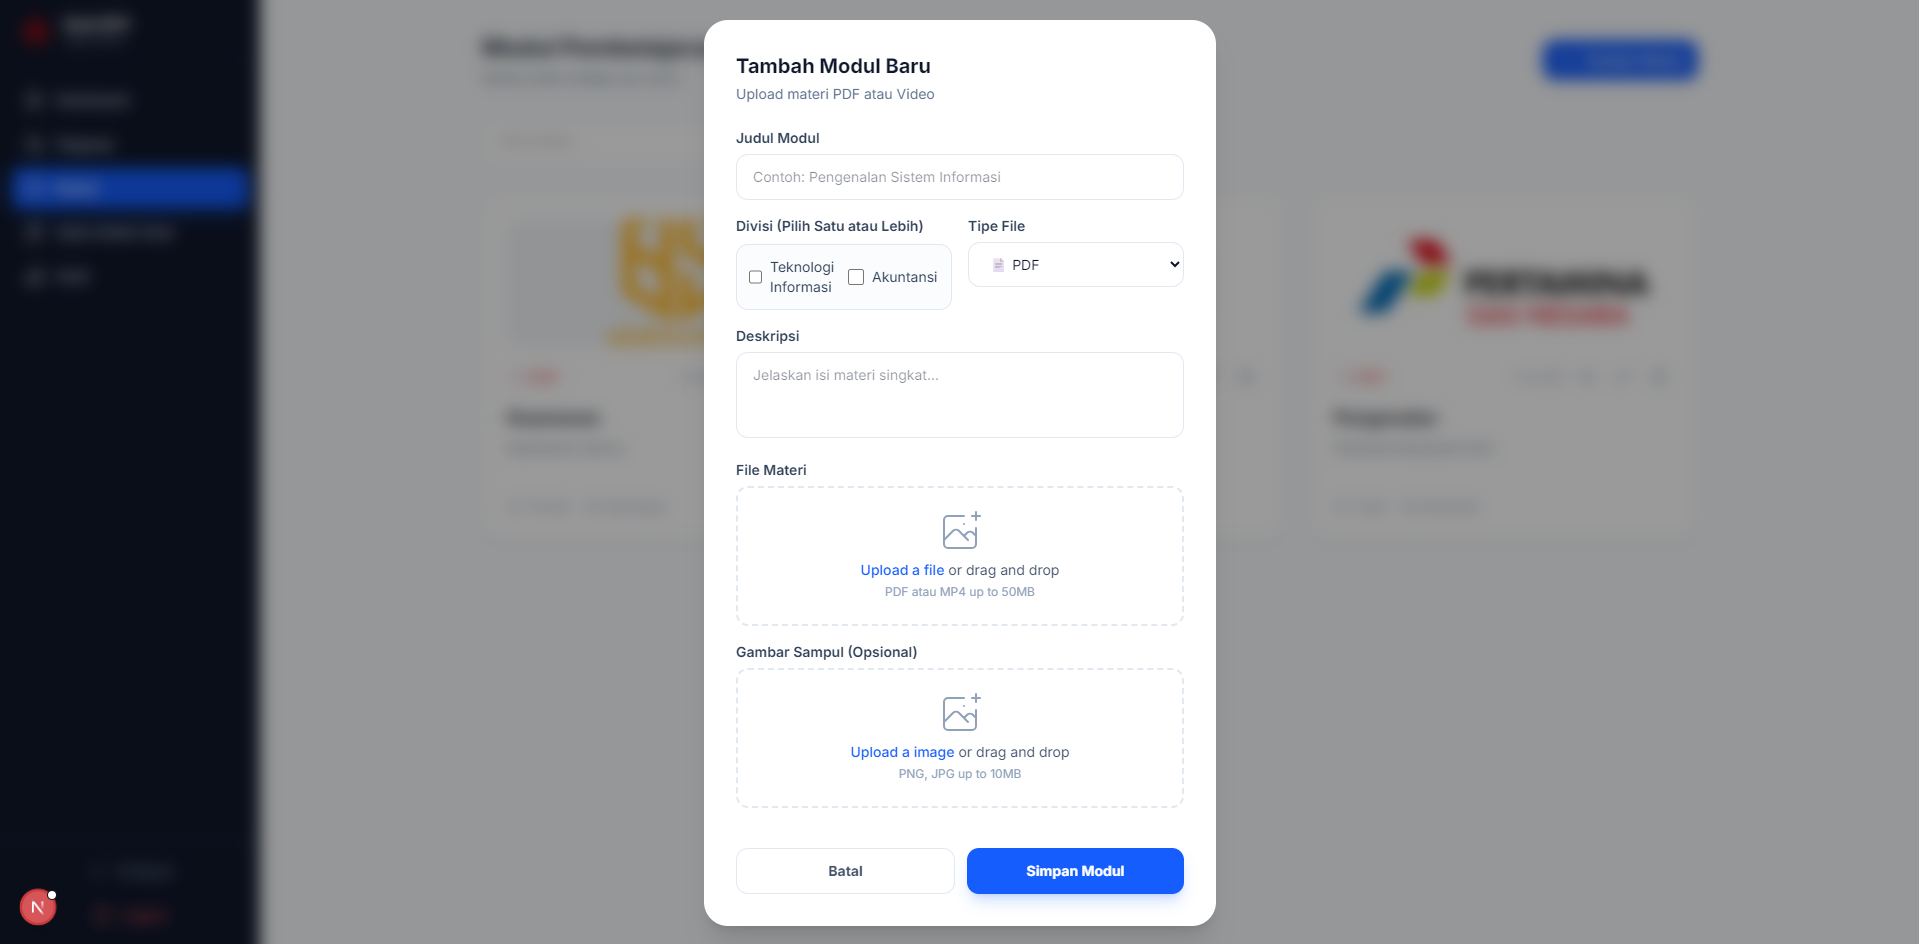
\includegraphics[width=0.75\textwidth]{image/fitur-tambah-modul.png}
    \caption{Form Unggah Modul Pelatihan Baru}
    \label{fig:tambah_modul}
\end{figure}

\subsection{Pembuatan Soal \& Kuis Evaluasi}
\begin{enumerate}
    \item Masuk ke menu \textbf{Kelola Ujian} pada \textit{sidebar} kiri.
    \item Klik \textbf{Buat Ujian Baru}, masukkan nama kuis, pilih modul terkait, tentukan KKM (skor minimal kelulusan), serta durasi pengerjaan.
    \item Klik detail ujian tersebut dan pilih \textbf{Tambah Soal}. Masukkan teks pertanyaan, pilihan jawaban A, B, C, dan D, serta tentukan pilihan yang merupakan kunci jawaban benar (Gambar \ref{fig:kelola_soal}).
\end{enumerate}

\begin{figure}[H]
    \centering
    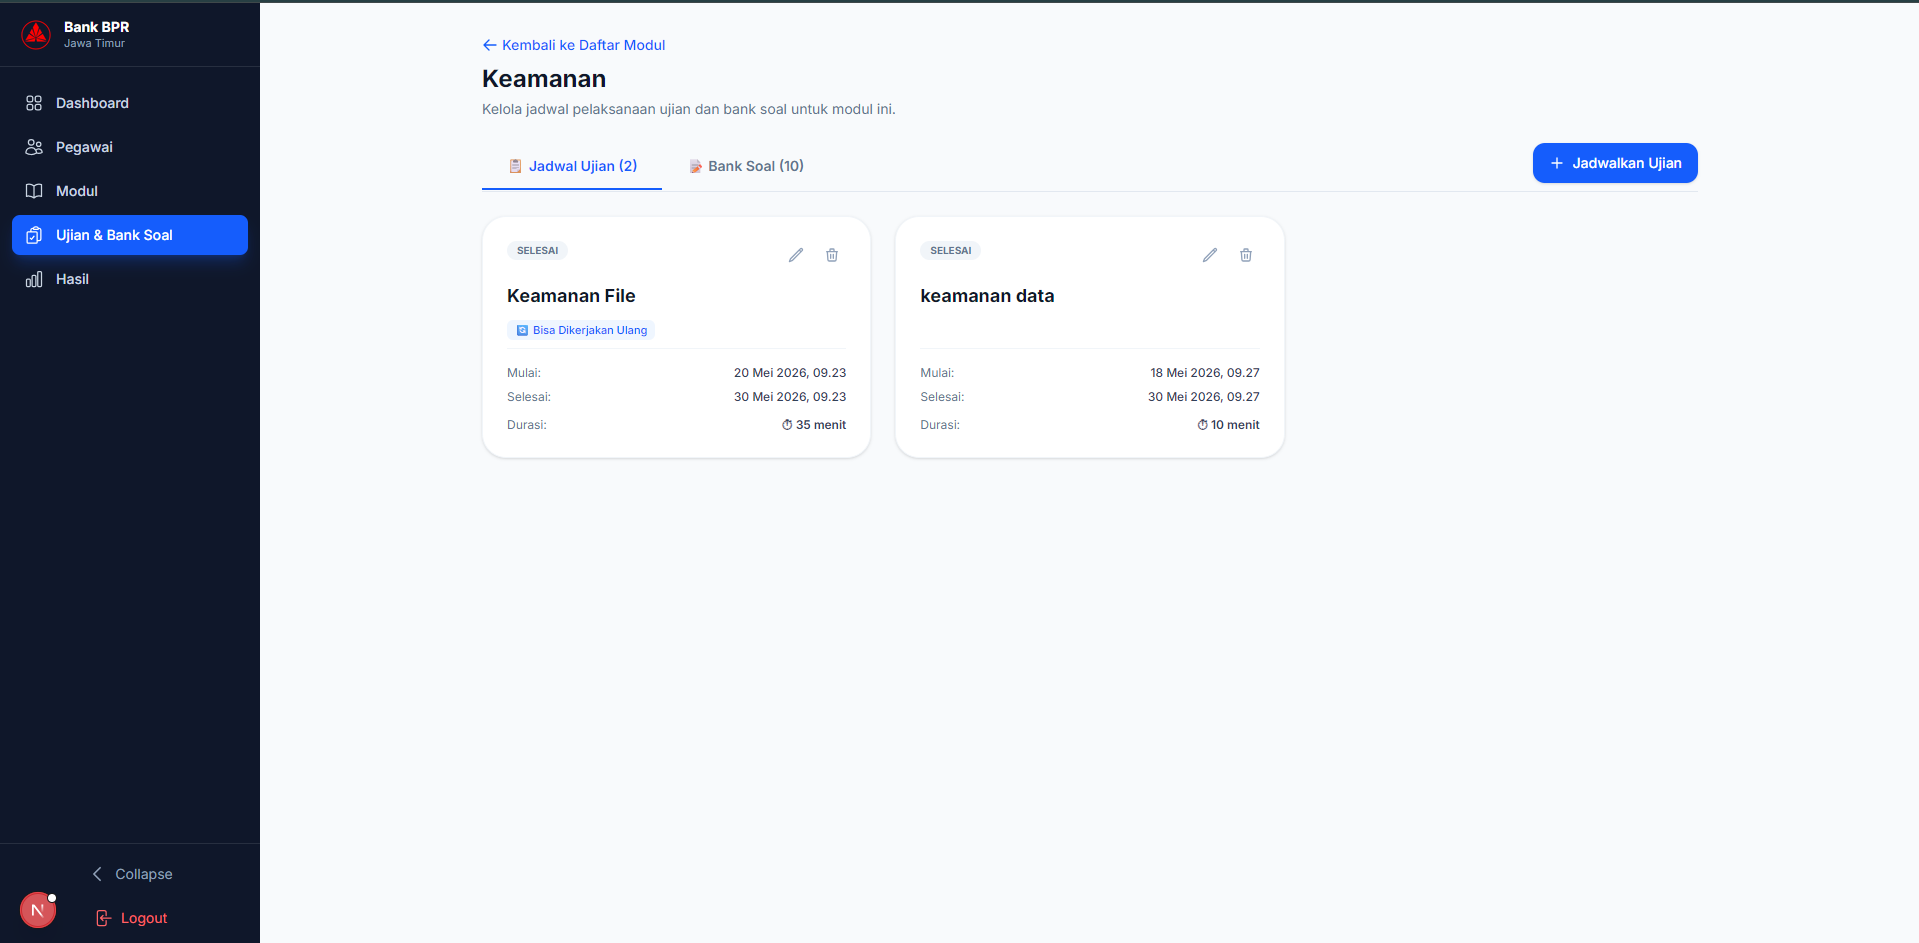
\includegraphics[width=0.85\textwidth]{image/halaman-kelola-soal-kuis.png}
    \caption{Halaman Kelola Soal Kuis Evaluasi}
    \label{fig:kelola_soal}
\end{figure}

\begin{figure}[H]
    \centering
    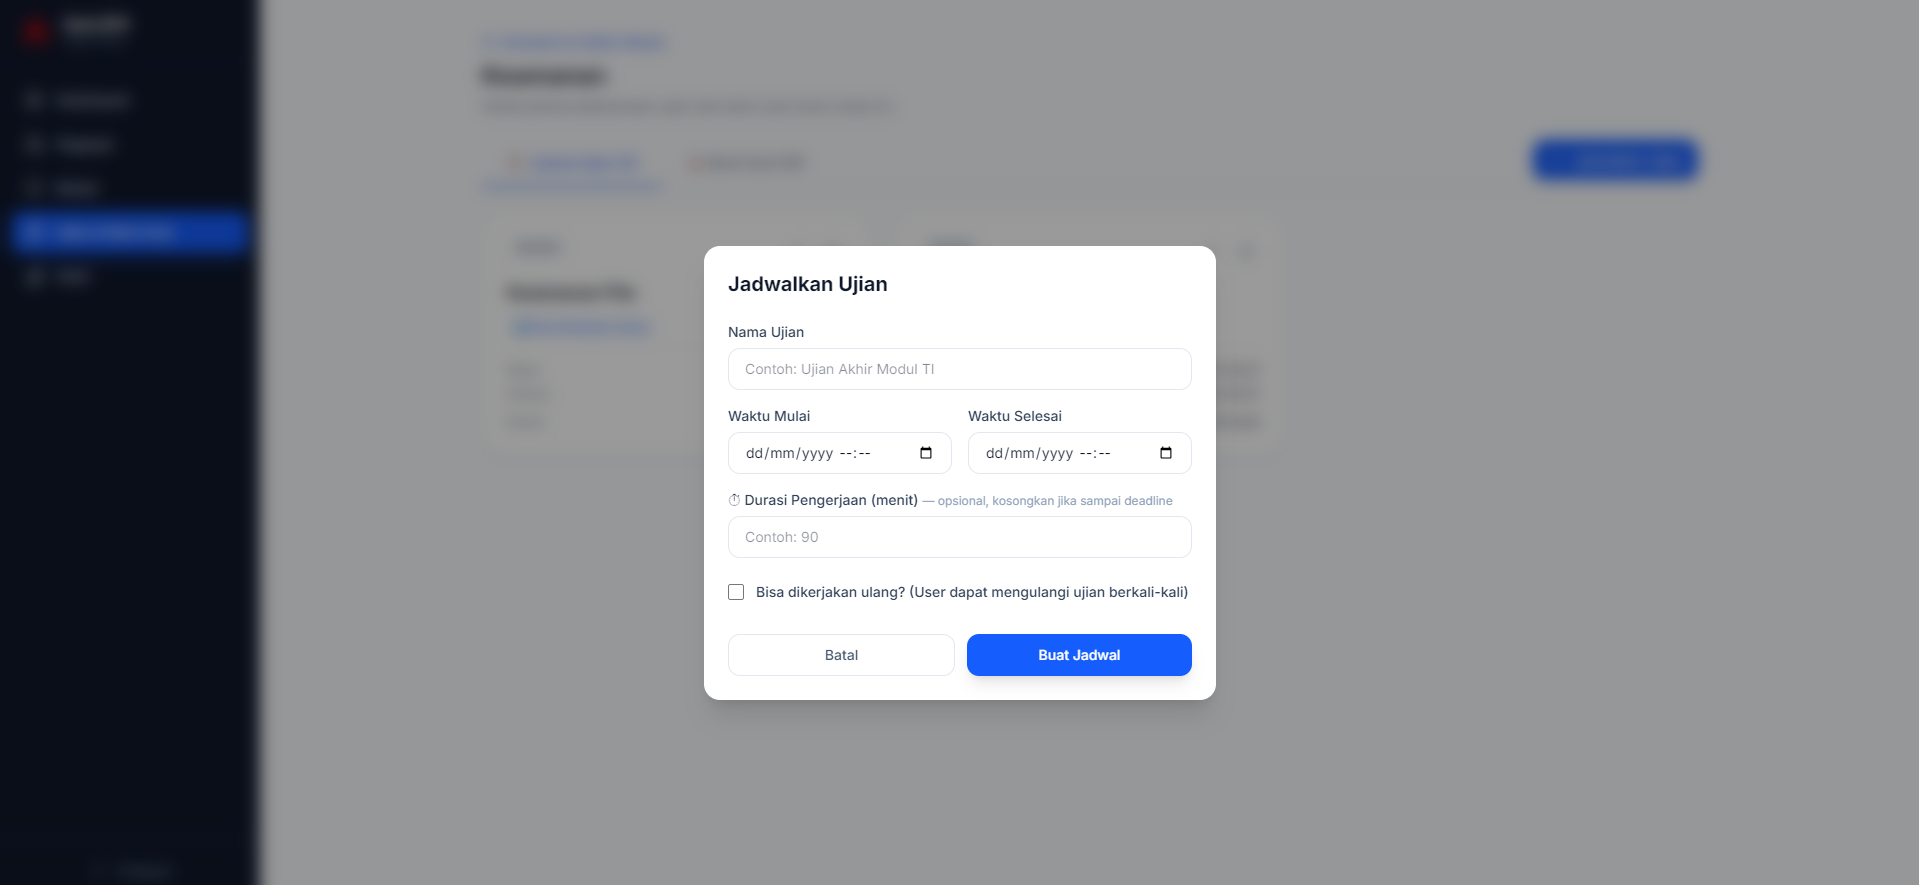
\includegraphics[width=0.85\textwidth]{image/web-kelola-soal.png}
    \caption{Detail Kelola Soal dan Kunci Jawaban}
    \label{fig:detail_soal}
\end{figure}

\subsection{Pemantauan Nilai \& Analitik}
\begin{enumerate}
    \item Masuk ke menu \textbf{Dashboard Nilai} atau \textbf{Pantau Nilai Karyawan} (Gambar \ref{fig:pantau_nilai}).
    \item Admin dapat memantau grafik rata-rata nilai kuis karyawan per divisi, melihat persentase kelulusan, serta menelusuri detail skor masing-masing karyawan.
    \item Data nilai kuis dapat diekspor ke format \textit{spreadsheet} Excel untuk bahan laporan bulanan kepada manajemen.
\end{enumerate}

\begin{figure}[H]
    \centering
    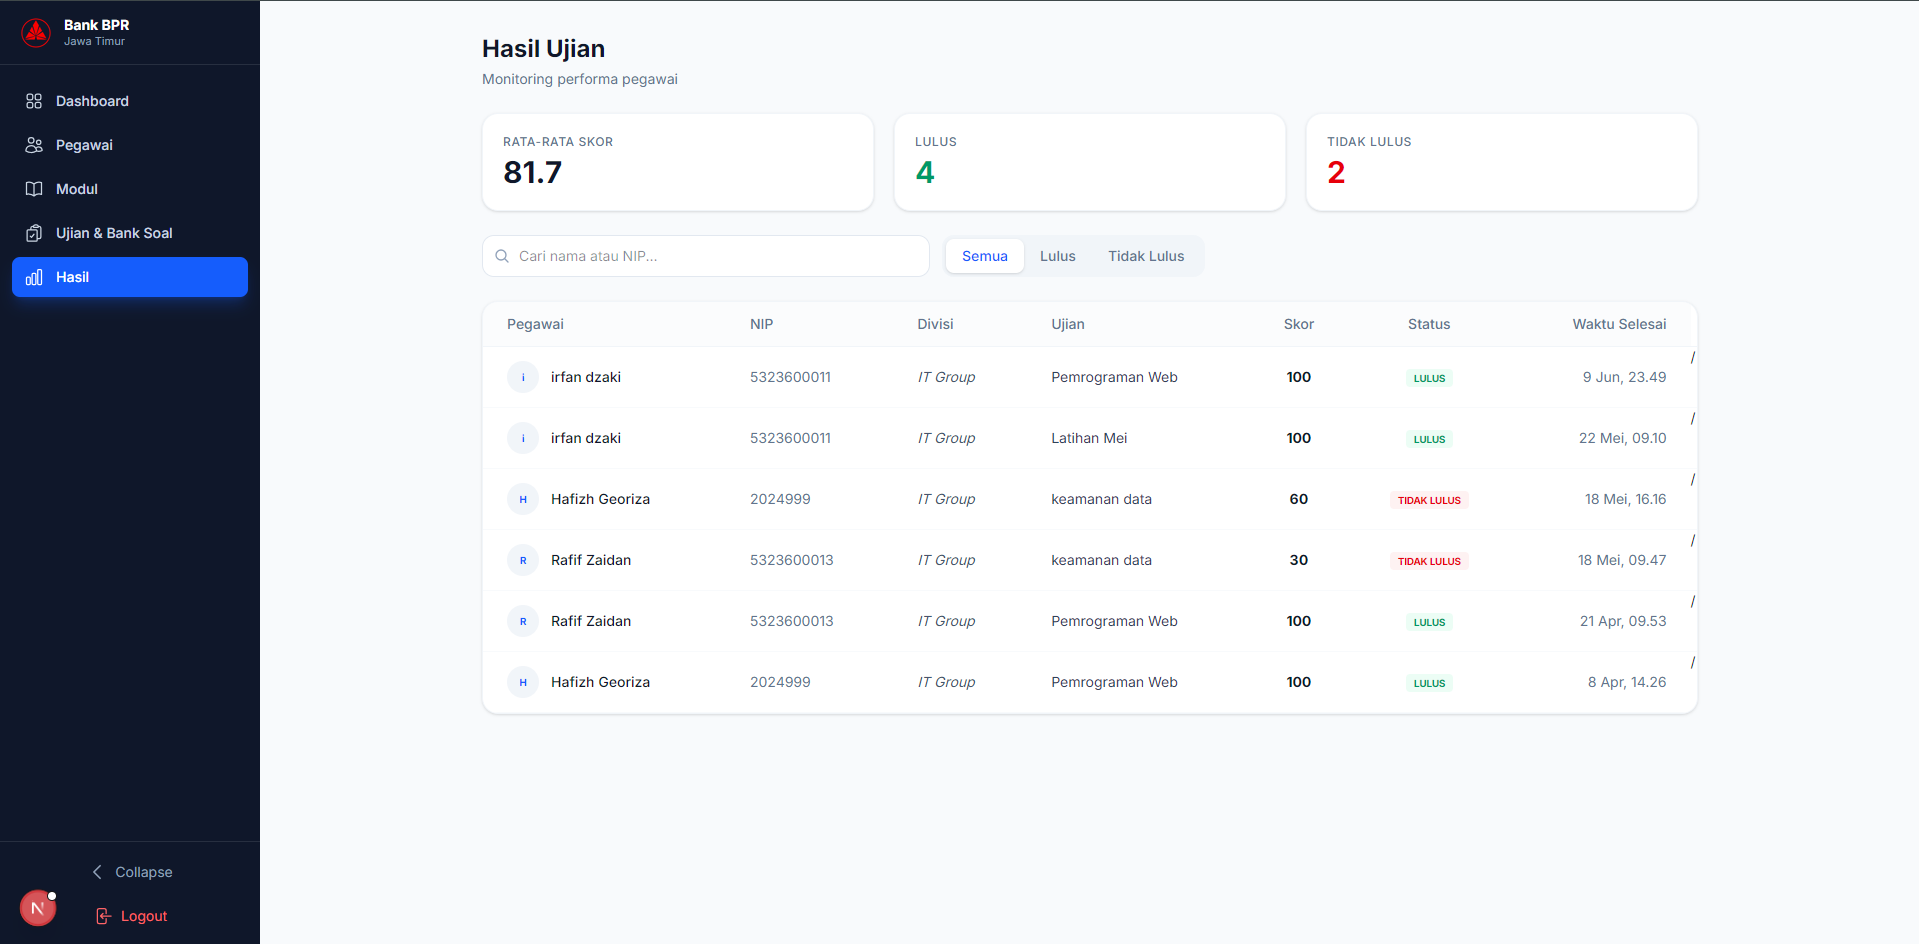
\includegraphics[width=0.85\textwidth]{image/halaman-pantau-nilai-karyawan.png}
    \caption{Halaman Pemantauan Nilai dan Analitik Karyawan}
    \label{fig:pantau_nilai}
\end{figure}

\newpage
\section{Panduan Aplikasi Mobile (Karyawan)}
Aplikasi Mobile digunakan oleh seluruh karyawan di PT. BPR Jatim untuk membaca modul pelatihan dan melaksanakan ujian kuis evaluasi.

\subsection{Pemasangan Aplikasi \& Login}
\begin{enumerate}
    \item Unduh berkas \textit{installer} aplikasi \textit{e-Learning} PT. BPR Jatim (.apk untuk Android / .ipa untuk iOS) dari repositori internal Divisi TI.
    \item Buka aplikasi, masukkan email atau NIP terdaftar serta kata sandi sementara yang diberikan oleh PSDM pada halaman Login (Gambar \ref{fig:login_mobile}).
    \item Lakukan penggantian kata sandi pada login pertama demi alasan keamanan.
\end{enumerate}

\begin{figure}[H]
    \centering
    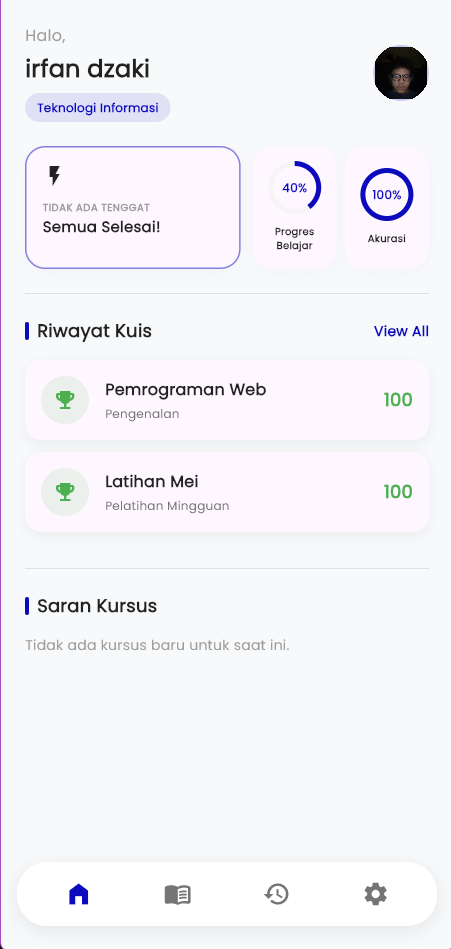
\includegraphics[width=0.35\textwidth]{image/halaman-login-mobile.png}
    \caption{Halaman Login Aplikasi Mobile Karyawan}
    \label{fig:login_mobile}
\end{figure}

\subsection{Dashboard \& Navigasi Aplikasi}
Setelah berhasil login, karyawan akan melihat halaman \textit{Dashboard} utama yang menampilkan katalog modul pelatihan sesuai divisi, jadwal kuis yang tersedia, serta riwayat nilai (Gambar \ref{fig:dashboard_mobile}).

\begin{figure}[H]
    \centering
    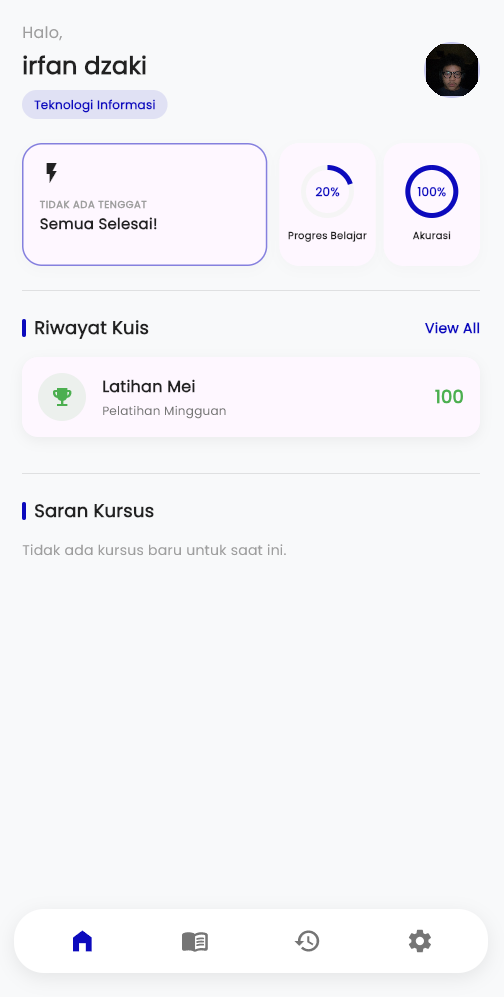
\includegraphics[width=0.35\textwidth]{image/mobile-dashboard.png}
    \caption{Halaman Dashboard Aplikasi Mobile Karyawan}
    \label{fig:dashboard_mobile}
\end{figure}

\subsection{Membaca Materi Pelatihan}
\begin{enumerate}
    \item Di halaman utama (\textit{Dashboard}), masuk ke tab \textbf{Pelatihan} untuk melihat daftar modul yang tersedia (Gambar \ref{fig:daftar_pelatihan}).
    \item Klik salah satu judul modul pelatihan yang tersedia untuk divisi Anda.
    \item Klik \textbf{Mulai Belajar}. Modul PDF akan terbuka di pembaca internal aplikasi sehingga karyawan dapat membaca halaman demi halaman secara langsung tanpa perlu mengunduh file (Gambar \ref{fig:baca_pdf}).
\end{enumerate}

\begin{figure}[H]
    \centering
    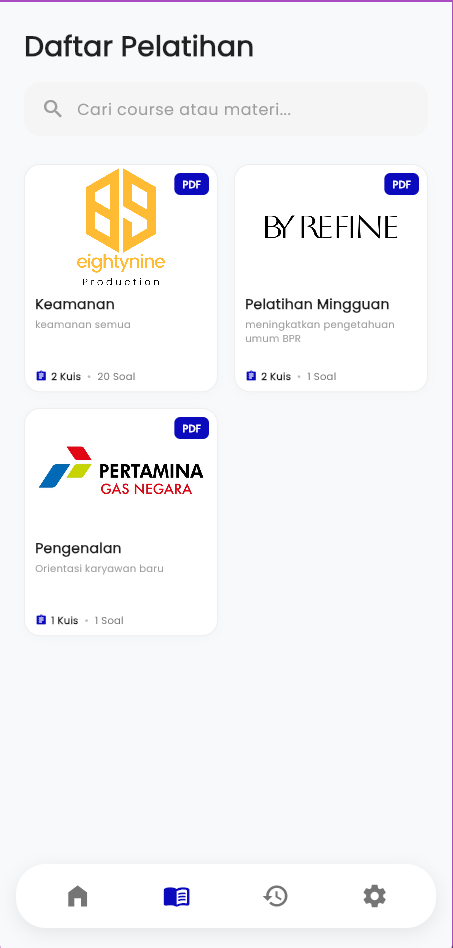
\includegraphics[width=0.35\textwidth]{image/halaman-daftar-pelatihan-mobile.png}
    \caption{Halaman Daftar Modul Pelatihan}
    \label{fig:daftar_pelatihan}
\end{figure}

\begin{figure}[H]
    \centering
    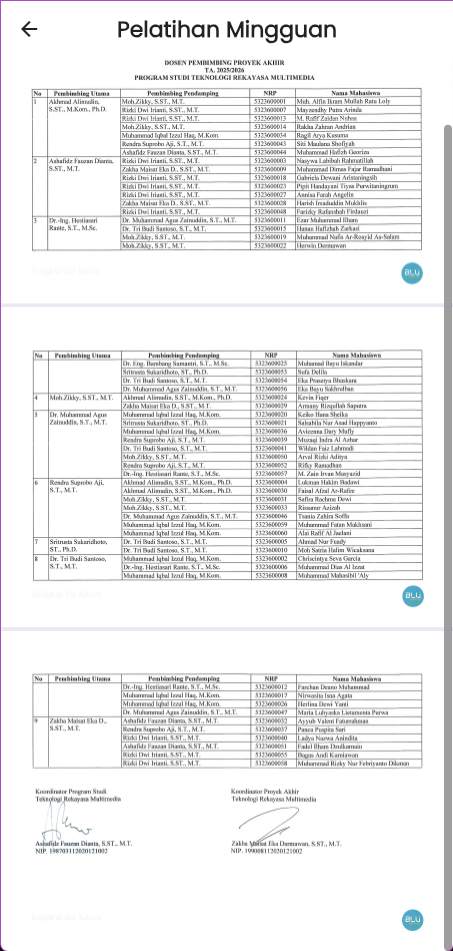
\includegraphics[width=0.35\textwidth]{image/halaman-pembaca-pdf.png}
    \caption{Tampilan Pembaca PDF Internal Aplikasi}
    \label{fig:baca_pdf}
\end{figure}

\subsection{Mengerjakan Kuis Evaluasi}
\begin{enumerate}
    \item Setelah selesai membaca modul, klik tombol \textbf{Kerjakan Kuis Evaluasi} di bagian bawah halaman materi, atau akses ujian melalui menu \textbf{Jadwal Kuis}.
    \item Klik \textbf{Mulai Ujian} (perhatikan batas waktu pengerjaan yang ditampilkan).
    \item Pilih jawaban yang paling tepat untuk masing-masing soal. Klik \textbf{Selanjutnya} untuk berpindah ke soal berikutnya (Gambar \ref{fig:kuis_mobile}).
    \item Pada soal terakhir, klik \textbf{Kirim Jawaban}. Skor Anda akan langsung ditampilkan di layar beserta status kelulusan (Lulus/Gagal).
\end{enumerate}

\begin{figure}[H]
    \centering
    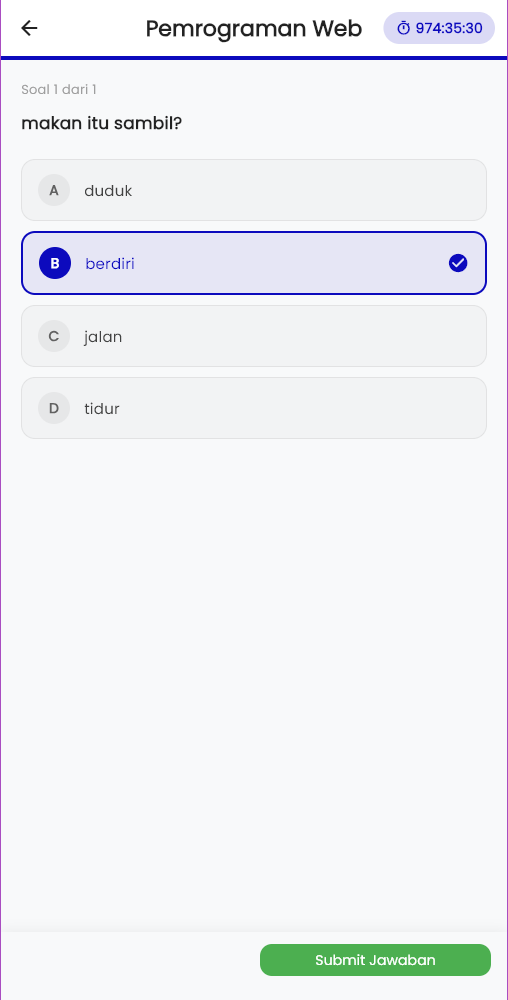
\includegraphics[width=0.35\textwidth]{image/mobile-kuis.png}
    \caption{Tampilan Pengerjaan Kuis Interaktif pada Aplikasi Mobile}
    \label{fig:kuis_mobile}
\end{figure}

\subsection{Melihat Riwayat Nilai}
Karyawan dapat melihat seluruh riwayat nilai kuis yang pernah dikerjakan melalui menu \textbf{Riwayat Nilai}. Halaman ini menampilkan daftar kuis beserta skor, tanggal pengerjaan, dan status kelulusan (Gambar \ref{fig:riwayat_nilai}).

\begin{figure}[H]
    \centering
    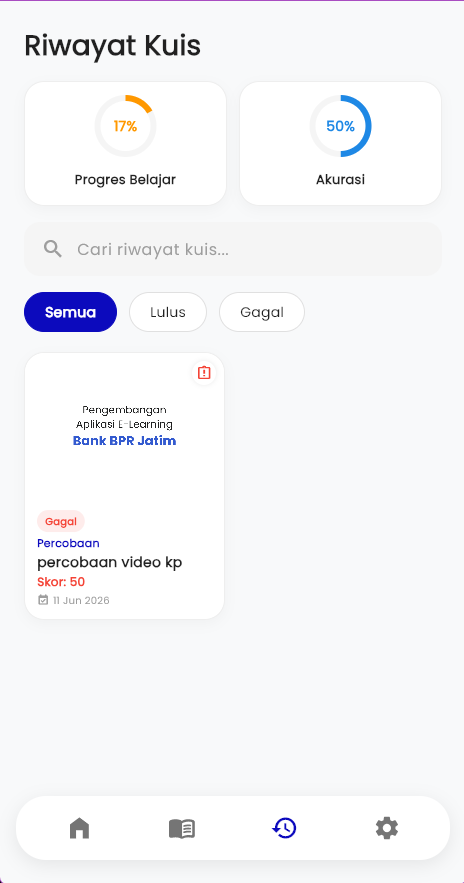
\includegraphics[width=0.35\textwidth]{image/halaman-riwayat-kuis-mobile.png}
    \caption{Halaman Riwayat Nilai Kuis Karyawan}
    \label{fig:riwayat_nilai}
\end{figure}
